\chapter{REVISÃO DE LITERATURA}

\section{Perfuração de Poços de Petróleo}

A perfuração de poços de petróleo constitui uma das etapas mais importantes das operações de exploração e produção, sendo responsável por estabelecer a comunicação entre a superfície e os reservatórios produtores. De modo geral, o poço é perfurado em fases sucessivas, definidas de acordo com as características geológicas das formações atravessadas e com a profundidade prevista do projeto. Ao término de cada fase, realiza-se a descida e cimentação de uma coluna de revestimento, cuja principal função é garantir a estabilidade do poço, prevenir o desmoronamento das formações, controlar a migração de fluidos e assegurar condições adequadas de segurança operacional ao longo da perfuração \cite{thomas2001}.

Dessa forma, a classificação dos revestimentos também possui grande importância no projeto de poços, uma vez que permite diferenciá-los de acordo com a função desempenhada em cada etapa da perfuração. De modo geral, os revestimentos podem ser classificados em condutor, de superfície, intermediário e de produção, conforme ilustrado na Figura \ref{fig:Figura01_revest}.

\begin{figure}[H]
	\centering
	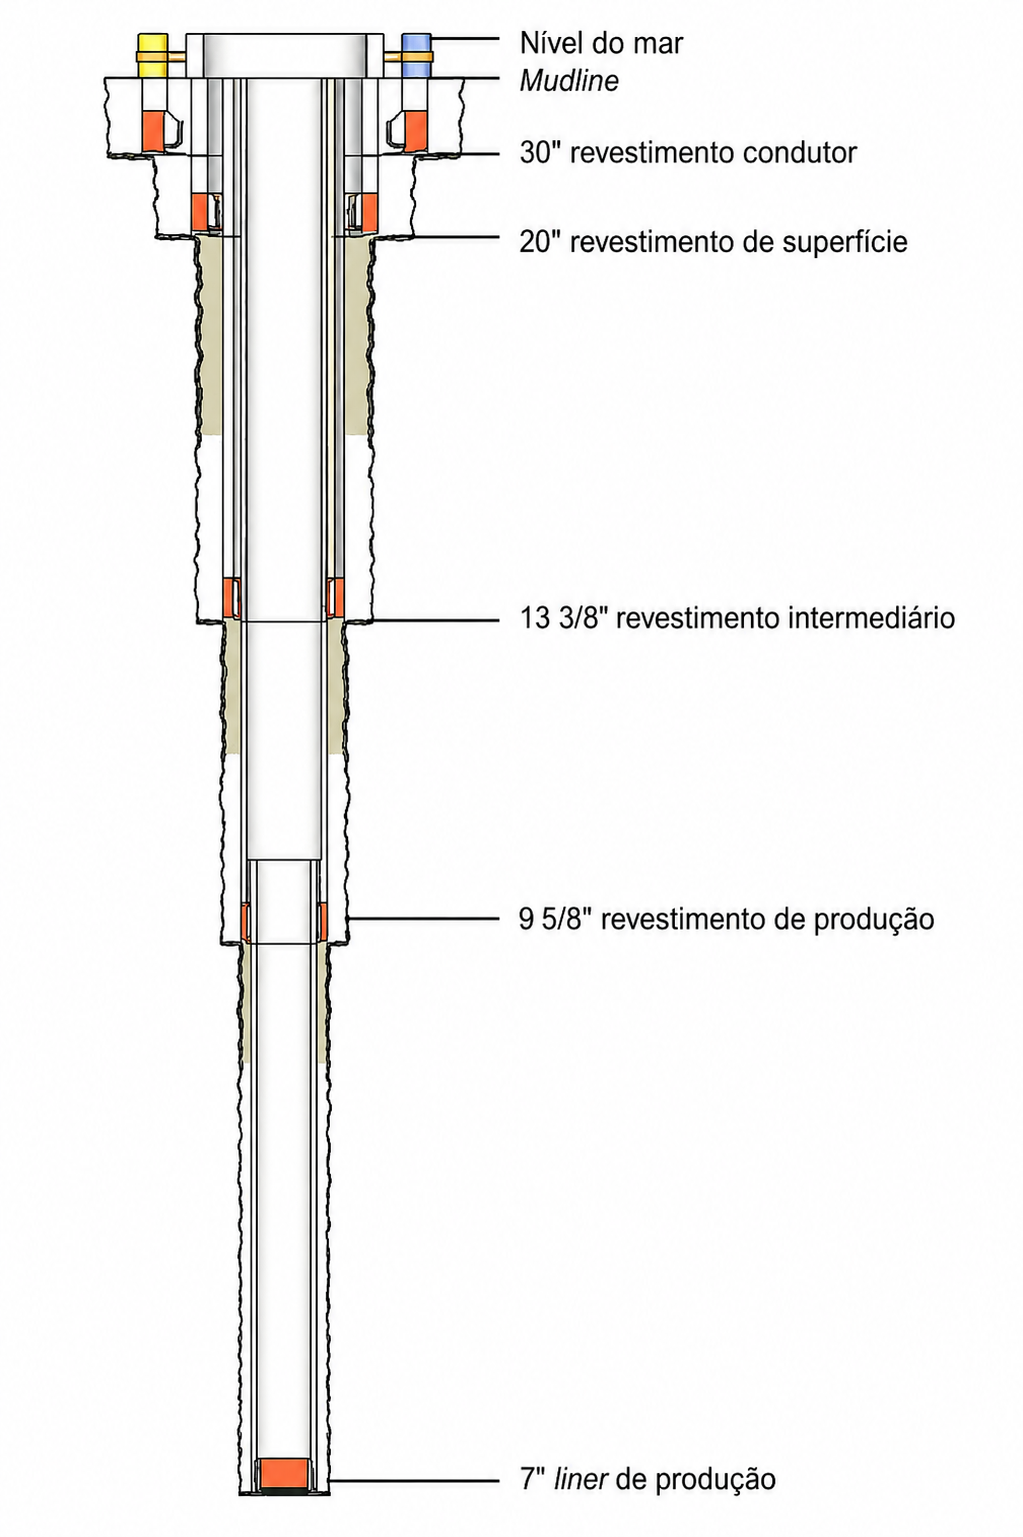
\includegraphics[width=0.5\linewidth]{figuras/Figura1_revest.png}
	\caption{Esquema de revestimento de poços. Fonte: \citeonline{rocha2009}}
	\label{fig:Figura01_revest}
\end{figure}

\citeonline{thomas2001} traz que o revestimento condutor corresponde à primeira coluna instalada no poço, sendo assentado a pequenas profundidades. Sua principal função é sustentar os sedimentos superficiais pouco consolidados, proporcionando estabilidade inicial à perfuração. A instalação desse revestimento pode ser realizada por cravação, jateamento ou perfuração seguida de cimentação, dependendo das condições geotécnicas do local.

O revestimento de superfície é descido após a perfuração das primeiras fases do poço e tem como objetivo proteger formações rasas, evitar o desmoronamento de zonas inconsolidadas e isolar aquíferos próximos à superfície. Além disso, essa coluna também atua como base de apoio para os equipamentos instalados na cabeça do poço e para as colunas subsequentes.

O revestimento intermediário tem como finalidade o isolamento de zonas específicas ao longo da perfuração, como formações instáveis, regiões com perda de circulação ou intervalos submetidos a pressões elevadas. Sequencialmente, o revestimento de produção é instalado na região do reservatório com a finalidade de permitir a produção de óleo e gás, além de garantir o isolamento entre as zonas produtoras e as demais formações atravessadas pelo poço. Em alguns casos, pode ser complementado pela utilização de liners, que correspondem a colunas de revestimento parcialmente ancoradas na coluna anterior.

Após o assentamento do revestimento, realiza-se a cimentação do poço, processo responsável pelo preenchimento do espaço anular entre o revestimento e as paredes da formação, garantindo a fixação da coluna e o isolamento hidráulico entre as zonas atravessadas \cite{rocha2009}. Em seguida, podem ser executadas operações de perfilagem e avaliação da formação, repetindo-se esse ciclo até a conclusão de todas as fases do poço.

\section{Instalação do revestimento condutor}

\subsection{Perfurado e cimentado}

\subsection{Base torpedo}

\subsection{Jateamento}

\subsection{Cravação por martelamento}

\section{Modelos constitutivos}

\section{Mohr-Coulomb}

\subsection{Drucker-Prager}

\subsection{Cam-clay}

\subsection{Norsand}

\section{Método dos Pontos Materiais}

\subsection{Two-phase single point}

\subsection{Algoritmo de contato}

\subsection{Algoritmo de corpo rígido}

\subsection{Malha móvel}

\section{Parâmetros do solo}

\subsection{CPTu}

\section{Estado da arte}